%% -*- coding:utf-8 -*-
\documentclass[ number=??
                ,series=lnls,
                ,isbn=xxx-x-xxxxxx-xx-x,
                ,url=http://langsci-press.org/catalog/book/14,
	        ,output=long    % long|short|inprep              
	        %,blackandwhite
	        %,smallfont
	        ,draftmode  
		  ]{LSP/langsci}                          

          
\hypersetup{pdfdisplaydoctitle=true}

\usepackage{xspace}
\newcommand{\latex}{\LaTeX\xspace}


\usepackage{embrac}

% just for the XeLaTeX logo
\usepackage{dtklogos}\newcommand{\xelatex}{\XeLaTeX\xspace}
\newcommand{\bibtex}{\BibTeX\xspace}

\usepackage{LSP/lsp-styles/avm}

\usepackage{lsp-makros}

\usepackage{german}\selectlanguage{USenglish}

\usepackage{LSP/lsp-styles/lsp-eng-hyp}

\usepackage{styles/abbrev}


      
% OT pointing hand
\usepackage{pifont}
\newcommand{\hand}{\ding{43}}

% OT tableaux                                                
\usepackage{pstricks,colortab}   

% DRS package by Alexis Dimitriadis
\usepackage{drs}

\usepackage{tabularx}

% AVMs
\usepackage{avm}
\avmfont{\sc} 
\avmvalfont{\it}

% command to fontify the type values of an avm 
\newcommand{\tpv}[1]{{\avmjvalfont #1}}

% command to fontify the type of an avm and avmspan it
\newcommand{\tp}[1]{\avmspan{\tpv{#1}}}


\usepackage{tikz-qtree}
% has strange side effects
%\tikzset{every tree node/.style={align=left, anchor=north}}
\tikzset{every roof node/.append style={inner sep=0.1pt,text height=2ex,text depth=0.3ex}}

\usepackage{jambox}


\setlength{\marginparwidth}{1.5cm}
\usepackage[textsize=tiny,textwidth=1.5cm]{todonotes}
\newcommand{\todostefan}[1]{\todo[color=green!40]{#1\xspace}}
\newcommand{\inlinetodostefan}[1]{\todo[color=green!40,inline]{{\normalsize #1}}}


% Chinese
\usepackage[indentfirst=false]{xeCJK}
\setCJKmainfont{SimSun}

% bidirectional text and support for Arabic/Persian
\newfontfamily\Parsifont[Script=Arabic]{XB Niloofar}
%\usepackage{bidi}
\usepackage{LSP/lsp-styles/lsp-bidi}
\newcommand{\PRL}[1]{\RL{\Parsifont #1}}
%\TeXXeTOff
\usepackage{LSP/lsp-styles/lsp-gb4e}

\def\exfont{\normalsize\itshape}

%% \iflsDraft
%% \proofmodetrue
%% \fi

% This is needed to allow for hyphenation in \texttt
% http://tex.stackexchange.com/questions/44361/how-to-automatically-hyphenate-within-texttt
% usually this is not required, but since we show index entries for packages in the margin and since
% the package names a re typeset in tt, we need the hyphenation.
\DeclareFontFamily{OT1}{cmtt}{\hyphenchar \font=-1}


\title{Language Science Press guidelines}  
\subtitle{General rules for editors, authors and \latex recommendations}
\BackTitle{Language Science Press guidelines}

\BackBody{This book contains the guidelines for Language Science Press authors and editors. For those who want
  to help keeping the production costs low and therefore decided to use \latex, it also contains
  descriptions of packages that can be used for typesetting trees, Attribute Value Matrices, OT-tableaux, Categorial
  Grammar proofs, LFG analyses, and much more. The setup of typesetting script with special fonts as
  for instance right to left scripts like Arabic is explained. The \latex chapter also contains sections
  concerning the efficient workflow in professional typesetting environments using \latex.

Stefan Müller is an experienced \latex user who has typeset four published books and several book
manuscripts and journal articles.
}

\dedication{This book is dedicated to everybody who cannot afford to buy books by profit oriented publishers.}

\typesetter{Stefan Müller}
\proofreader{Test T.\ Tester, Test T.\ Tester, Test T.\ Tester, Test T.\ Tester, Test T.\ Tester, Test T.\ Tester,}

\author{Stefan Müller and Martin Haspelmath}



\makeatletter
\def\verbatim@font{\scriptsize\ttfamily}
\makeatother
         
%\renewcommand{\eachwordone}{\it}
%\renewcommand{\exfont}{\it}
%\def\exfont{\it}

\begin{document}               
         
                                                                           
                                  
\maketitle                

%\frontmatter

\chapter*{Preface}

%\lipsum[3-10]  

This book has several purposes: it describes the editorial process and contains guidelines with some style rules for all
authors. In addition it contains a part for authors who use \latex or who want to learn \latex in order to
support \lsp. The \latex part is also a reference for those who volunteered to help typesetting
manuscripts that were not submitted in \latex. See \citew{MuellerOA} and \citew{MH2013a} for an overview of the
general setup of the project.

\section*{Acknowledgements}



%% David Reitter danke ich für die \LaTeX"=Makros für Combinatorial
%% Categorial Grammar, Mary Dalrymple und Jonas Kuhn für die LFG"=Makros und Beispielstrukturen, und
%% Laura Kallmeyer für die \LaTeX"=Quelltexte der meisten TAG"=Analysen. Ohne diese
%% Originalmakros/-texte wären die Darstellungen in den jeweiligen Kapiteln sicher nicht halb so schön
%% geworden. 

This book is typeset with \xelatex. We thank the \latex developers for their work and the members of
the \textit{German Language TeX Users Group Communication List} and those replying at \url{http://tex.stackexchange.com} for many usefull hints and suggestions.

We thank Matthias Hüning\aimention{Matthias H{\"u}ning} for comments on an earlier version of this document and Corinna Handschuh\aimention{Corinna Handschuh}
and Francesco Cangemi\aimention{Francesco Cangemi} for being the first to use the new \latex classes and providing feedback
to us.

\bigskip

\noindent
Berlin, \today\hfill Stefan Müller \& Martin Haspelmath


\tableofcontents      

\mainmatter         

%% -*- coding:utf-8 -*-
\chapter{General information on Language Science Press}


\section{Background and motivation}

Language Science Press is a book imprint that publishes high-quality books in the field of academic
linguistics. It was founded in 2013, growing out of the initiative ``Open-Access Books for
Linguistics'' (OALI) that was started by Stefan Müller (and other linguists at FU Berlin) and joined
by Martin Haspelmath. After its first launch in August 2012, it quickly found several hundred
supporters from various subfields of linguistics and a range of different countries, including some
very prominent linguists.

The problem to which this initiative responded was the increasing cost of linguistics books, which
is in increasingly stark contrast with the ease with which files can be shared
\citep{MuellerOA}. More and more, it seems that most of what the traditional publishers add to the
scientists' work is the prestige of an imprint label \citep{Haspelmath2012a}, but this is something
that is ultimately created by the scientists as well.

Thus, we decided to found a new imprint (\lsp) dedicated to publishing high-quality books which exist primarily in electronic form. Printed copies will be available through print-on-demand services. This imprint will be owned and run by scholars, and neither authors nor readers will be charged. The required work (reviewing, proofreading, typesetting) will be organized and carried out by the scholars themselves.

Language Science Press is associated with the FU Berlin and is directed by Stefan Müller and Martin Haspelmath.

In December 2013, the DFG (Deutsche Forschungsgemeinschaft) awarded us a substantial amount of funding, which allows us to employ a number of people to develop our activities in various domains.


%% \section{Set Up and Responsibilities}

%% Language Science Press works with Open Monograph Press’s (OMP) management software.
%% (more details will follow later)

\section{Strategy}

We are working with the assumption that book publication can nowadays be organized in a much cheaper and more efficient way. Essentially, to publish high-quality books, the following tasks need to be carried out:

\begin{enumerate}
\item[(i)] manuscript reviewing
\item[(ii)] typesetting
\item[(iii)] proofreading
\item[(iv)] overall coordination
\item[(v)] hosting
\end{enumerate}

We are assuming that (i) can be done by the series editors without much help from the coordinators,
that (ii) can be done by the authors (initially with help from the coordinators and later with help
from the series editors), that (iii) can be done by volunteers from the LangSci community, and that
the work for (iv) will get less and less as we develop a routine. The fifth point, hosting, is taken
care of by the FU Berlin.

The main challenges are (ii) typesetting by the authors and (iv) making the coordination tasks
slim. Professional typesetting requires the use of LaTeX, and while an increasing number of
linguists is familiar with this typesetting software, many others are not. But we trust that there
will be a sufficient number of linguists willing to invest the effort to do the LaTeX typesetting
(or to find someone to do it for them). This Guidelines text provides the necessary information
about \latex classes.


To reduce the amount of coordination that is required, series editors and authors will have to conform very strictly to our standard procedures. While commercial publishers with permanent staff members can afford to allow deviations from the general rules, this is not really possible with our model. Authors and editors who find our procedures too inflexible will have to choose alternative publication outlets. The present Guidelines set out the rules that editors and authors must obey if they want to publish with Language Science Press.



\section{Responsibilities}

All books published by Language Science Press appear in book series, which are managed by a Series
Editor (or a team of Editors). The Series Editors are in charge of the reviewing and the coordination of the production of
the books in their series. The overall coordination of the Press is in the hands of the Press
Directors Stefan Müller and Martin Haspelmath.

\subsection{Advisory board}

The Advisory Board was particularly important in the early stage of Language Science Press, when there were few series. Its task was and is to assess proposals for new series, as well as to give respectability to the whole enterprise.


\subsection{Series and editorial boards}

Each series is run by a team of Series Editors, who bear full responsibility for manuscript
reviewing, selection and coordination of production. The Series Editors are generally supported by
an Editorial Board, i.\,e.\ 5--25 colleagues from various places whose expertise falls in the area of
the series. Editorial Board members should be willing to review at least one book manuscript per
year.

\subsection{Open Monograph Press and CEDIS}

Language Science Press uses the Public Knowledge Project’s software \emph{Open Monograph Press} (OMP),
which was specifically designed for open-access publishers. We are in regular contact with OMP's
software developers.

The OMP software is hosted by the CeDiS, who also provides support for authors and editors.


\subsection{The library of the Freie Universität Berlin}

The library of the Freie Universität Berlin is in charge of storing the published versions of the
books on the document server of the Freie Universität and i sresponsible for providing
bibliographical metadata for the books. 

%% \subsection{Design}

%% The design of the Language Science Press books (text design and cover design) has been done by professional designer Ulrike Harbort.


\section{Open access and licence}

All Language Science Press books are published with open access, i.\,e.\ they can be downloaded free of
charge. All rights (copyrights, translation rights) remain with the author. 

By default, \lsp books are published with a Creative Commons CC-BY licence\footnote{ 
  Currently \url{http://creativecommons.org/licenses/by/4.0/}, 16.02.2014.
} (see \citew{Shieber2012a} for details
of what this means and why it is the preferred licence for scientific papers and books). The CC-BY
license allows for free reuse of the material in the book, including commercial uses as for instance
edited volumes that contain parts of the book licensed under CC-BY. The only condition is that the
work is properly attributed to the author/authors. The CC-BY license guarantees maximal distribution
of the material.

In certain situations, a CC-BY license is not possible. For instance if \lsp publishes a translation of a
book that already appeared with another publisher. In such situations the books will be published
under the more restrictive CC-BY-ND license\footnote{
Currently \url{http://creativecommons.org/licenses/by-nd/4.0/}, 16.02.2014.
}, which forbids to change the material (NoDerivatives) and hence guarantees that
the rights of the original publisher are not violated by somebody translating the work back into the
original language and distributing the book commercially or non-commercially.


%(more details will follow later)


\section{Print on demand}

There will be a print-on-demand service connected to the Language Science Press website. Thus, it will also possible to purchase printed copies of the books.



%      <!-- Local IspellDict: en_US-w_accents -->

%% -*- coding:utf-8 -*-
\documentclass[ number=??
                ,series=lnls,
                ,isbn=000-0-000000-00-0,
                ,url=http://langsci-press.org/catalog/book/0,
	        ,output=long    % long|short|inprep              
	        %,blackandwhite
	        %,smallfont
	        ,draftmode  
		  ]{LSP/langsci}                          
\author{Stefan Müller and Sebastian Nordhoff}
\title{Guidelines for e}
\begin{document}
\chapter{Guidelines for editors}

\section{Decision structure}


Each \lsp series has a team of Series Editors, who decide which books are accepted for the
series. There can be up to three Series Editors per series; if more people are involved at the top
level, one or two have to be the Chief Editors, and the others are Consulting Editors (or simply
Editors).

In addition, each book series normally has an Editoral Board of 10--35 members. The Editorial Board
members advise the Series Editors in various ways concerning the series, in particular by writing
manuscript reviews. However, the list of names of the Editoral Board also serves to indicate the
kind of orientation that the series is inteded to take, and not least to give prestige to the
series. Editorial Board membership is normally for a period of three years (renewable).

For the first seven books in each series, acceptance is conditional on approval by the Press
Coordinators. This ensures that there is agreement between the Series Editors and the Press
Coordinators on the level of quality of the series. This is important to ensure a uniformly high
quality of all series.

\section{Series web pages}

Each series has a homepage, which lists the Series Editors, the Editorial Board members (with
affiliation), and contains an Aims and Scope statement.

All published books are listed on the page of the series. (They can also be found elsewhere on the
\lsp site, e.g. under ``\href{http://langsci-press.org/catalog}{Catalog}''.) This page may also list
forthcoming books, i.e. books which have been accepted, revised and approved and are at the
production stage.

As soon as a book has been accepted and approved, it can be put on the website as ``forthcoming'',
with the bibliographical information, but without the actual downloadable file. This will serve the
purpose of advance publicity.

(more details will follow later)

\section{Types of book manuscripts}

Language Science Press books may be monographs or edited volumes in English, German, French, Spanish,
and Portugese. Which languages are accepted depends on the particular series.

The manuscripts should have a size of at least 80 pages and at most 800 pages.
% We decided to remove the upper limit. IDS grammar has 2500 pages, what about dictionaries?
There are no technical reasons for excluding shorter and longer manuscripts, but such manuscripts
are not clearly within the scope of what readers would expect when they hear ``book''. Shorter works
are perhaps better published as journal articles, and longer works are difficult to organize a
serious reviewing process for.

(more details will follow later)


\section{Submission and reviewing procedure (monographs)}

Book manuscripts are officially submitted by entering them into the OMP system. Of course,
informal preliminary submission (by e-mail or by some file sharing mechanism) is
possible. Official submission implies that all Series Editors (as well as the Press Coordinators)
are informed of the submission, if the submission is done without OMP.


In a next step, the manuscript is made available to the reviewers via the OMP system (initially,
while not everyone is familiar with it, this can be done informally, e.g. by e-mail). For each book
manuscript, at least two reviews are solicited, within a time frame of two months. The reviews are
made available to the Press Coordinators. The Series Editors may override the recommendations of the
reviewers, but if all reviewers are mostly negative, this needs to be justified to the Press
Coordinators.

If a reviewer does not react even after three months, it is recommended that the Series Editors
solicit at least one additional review. If within six months after submission fewer than two reviews
are returned, the manuscript counts as rejected.

If a manuscript was rejected, the same author may submit another manuscript a year after the
submission of the rejected manuscript. The new manuscript may be similar to the originally submitted
manuscript, so the author may think of this as a ``resubmission''. However, there is no official
resubmission procedure in Language Science Press, and there is no ``revise and resubmit'' decision.

Note that Language Science Press does not issue ``contracts'' on the basis of book proposals, like
other publishers do. Book proposals may be discussed informally with the Series Editors, and the
Editors may informally encourage the author to submit a book on the basis of an informal book
proposal, but none of this has any binding status.

\section{Submission and reviewing procedure (edited volumes)}

For edited volumes, the Series Editors may adopt the same procedure as for monographs, or
alternatively they may accept the volume without review, i.e. they delegate the quality control to
the book editor. However, this is possible only if the papers underwent a comments \& revision
process, and if upon submission, the book editor gives a full account of the comments \& revision
procedure to the Series Editors. In such a case, a book manuscript may be accepted without revision.

\section{Acceptance}

On the basis of the reviewers' reports, the Series Editors decide whether the book is accepted for
the series or not.

If revisions are needed or recommended (as is likely to be the case), then this is a preliminary
acceptance, conditional on proper execution of revisions. However, peliminary acceptance means that
an author is allowed to cite the book as ``to appear with Language Science Press''.

Upon acceptance of a book manuscript, not only the author and the Press Coordinators, but also all
the other Series Editors are informed, so that they stay informed of developments within the entire
Press (see Section~\ref{sec-editors-information}).
%\todostefan{This should be done by OMP.}


\section{Revision}

If a book manuscript is accepted, the Series Editors convey the reviews and their own comments to
the author, and the author is asked to revise the manuscript.

The Series Editors may specify some Required Changes on which the definitive acceptance is
conditional. The Required Changes may only be highly specific changes that are not very
time-consuming. Vague proposals for changes (``the approach needs to be more firmly grounded in
theory'', etc.), or changes that require a lot of additional work, are not acceptable as Required Changes.

Apart from the Required Changes, authors may choose to ignore recommended changes, but these cases
need to be justified to the Series Editors. In the case of a serious disagreement between author and
Series Editors, the Press Coordinators are ready to mediate.

If the changes are made as requested the book will receive Definitive Acceptance.  The revision
stage includes proofreading. Like the revision of the content, this is the Series Editors'
responsibility, but the \lsp Community will be able to help with this. (Details will follow later.)

\section{Production}

Once the revised version of a manuscript has been returned by the author and Definitively Accepted
by the Series Editors, production can begin.

\subsection{Rough typesetting}

LaTeX styles are applied, figures are created in the proper way, etc.

\subsection{Formal contract}

At this stage, the author signs a contract with the FU Berlin (which is reponsible for hosting and permanent archiving) about the legal publication of the book. The contract form can be downloaded from the following page:

http://edocs.fu-berlin.de/docs/content/main/autoren/vertraege.xml?lang=en

Basically only the author's address needs to be filled in, as well as the book title and the URL (http://langsci-press.org/catalog/book/...).

This contract is necessary for the application for an ISBN number, which is needed for typesetting.

\subsection{Metadata and catalog}

The Series Editors/Authors enter the following metadata about the book into OMP:
\begin{itemize}
\item book synopsis (for the web page and back cover)
\item author bio
\item add keywords, regions, languages, and so on
\end{itemize}
The book also needs to be assigned to a category. At the moment, we are working with the following
categories:
\begin{itemize}
\item Phonetics and Phonology Phonetics
\begin{itemize}
\item Phonetics
\item Phonology
\end{itemize}
\item Morphology
\item Syntax
\item Semantics
\item Pragmatics
\item Historical Linguistics
\begin{itemize}
\item Comparative Historical Linguistics 
\end{itemize}
\item Typology
\end{itemize}
Once all these things have been taken care of, the book can be announced in the catalog as ``forthcoming''.

\subsection{Community proofreading/commenting}

(Details will follow later. Maybe at this stage the manuscript will already be made available publicly, so that anyone can make comments.)

%\todostefan{added commenting}

\subsection{Revised typesetting}

If necessary authors may revise their text taking into account the comments from the community proofreading stage.

\subsection{Final check}

Series Editors and Press Coordinators do a final check. If further changes are necessary, the
typesetting is adjusted again.


\subsection{Publication}

Once author, Series Editors AND Press Coordinators have given their imprimatur, the book is published by the Press Coordinators.


\section{Editors' information}
\label{sec-editors-information}

There will be two newsletters per month to inform all series editors about new submissions, accepted
manuscripts, published books and other news. 
\end{document}
%% -*- coding:utf-8 -*-
\chapter{Style rules for authors}

Authors can submit books after registering as an author at
\url{http://langsci-press.org/user/register}. \lsp only publishes books that are assigned to a
series. It is suggested that authors contact the series editor informally before an official submission.
The submission has to be in PDF format to make proper
reviewing (reference to page numbers) possible. The first submission does not have to correspond to
the format specification that is outlined in this chapter, but if it does this is good since it
enables series editors to get some idea about the length of the book and so on. If authors submit an
almost final version in the proper layout, this speeds up production, since comments on form can be
provided in the first reviewing steps.


The following sections describe the layout of various items that play a role in typesetting. Many of
these things are covered automatically by the Word Template\footnote{
\url{https://github.com/langsci/word}, 19.02.2014.
} or by our \latex classes\footnote{
\url{https://github.com/langsci/latex}, 19.02.2014.
}. Authors who start a new book project are strongly recommended to use \latex from the very beginning.


\section{Front matter}
The front matter of \lsp books is structured as follows
\begin{itemize}
 \item optional dedication
 \item obligatory table of contents 
 \item obligatory Notes on contributors (only in edited volumes)
 \item optional notational conventions
 \item optional acknowledgements
 \item optional preface
 \item optional list of abbreviations
 \item no lists of figures or lists of tables!
\end{itemize}

\section{Back matter}
The back matter is structured as follows:

\begin{itemize}
 \item optional Appendix A
 \item optional Appendix B etc
 \item optional further appendices
 \item obligatory Bibliography
 \item obligatory Author index
 \item optional Language index (advisable if the book talks about a larger number of languages)
 \item obligatory Subject index
 
\end{itemize}


\section{Chapters}

Every book is divided into consecutively numbered chapters. In addition to chapters, a book may also
group chapters into parts (numbered I, II, III). %Chapter numbering is not restarted within parts.




\section{Sections and headings}

All sections (= parts of chapters) have headings and are numbered. Authors may use structures with up to
six levels, i.e. there may be a section with the number 1.2.3.4.5.6.\footnote{
  See page~\pageref{sec-Chinese} for an actual use of subsubsections.%
} However, such elaborated
structures may be difficult for the readers, so there should be a good motivation for going beyond
three or four levels.

Sections and subsections must be minimally two and must be exhaustive. This means that all text in a chapter
must belong to some section, all text within a section must belong to some subsection and so on. A
short intro paragraph is allowed by way of exception, as in the current Section 3 (see the intro
paragraph above Section 3.1).\todo{würde ich nicht erlauben SN}

Please do not change the capitalization of words when they are used in titles. 
% Please write the headings of chapters and sections without special capitalization.
This also applies
to the title (and subtitle) of the book itself and to the bibliographical references. Language
Science Press never uses special capitalization.
% , as it potentially introduces ambiguity, and there are no clear rules for special capitalization in English anyway.

\section{Italics, small caps, and punctuation marks}

\textbf{Boldface} is generally restricted to section headings.
\textit{Italics} are used for the following purposes:
\begin{enumerate}
\item for all object-language forms that are cited within the text or in set-off examples (e.g. in (2) and (4) below), unless they are written in IPA or otherwise in the context of the discussion of sounds;
\item  when a technical term is referred to, e.g. ``the term \textit{quotative} is not appropriate here'', or ``I call this construction \textit{quotative}''. In such contexts, English technical terms are thus treated like object-language forms;
\item for emphasis of a particular word that is not a technical term (``This is possible here, but \textit{only} here'').
\textsc{Small caps} are used for highlighting important terms on first mention, e.g.
\end{enumerate}
\ea
On this basis, the two main alignment types, namely \textsc{nominative-accusative} and \textsc{ergative-absolutive}, are distinguished.
\z

Small caps are also used for category abbreviations in interlinear glossing, and they may be used to indicate stress or focusing in example sentences:

\ea 
John called Mary a Republican and then \textsc{she} insulted \textsc{him}.
\z


% To emphasize terms, please use \emph{italics}. Boldface should be avoided if
% possible. New terms should be set in {\sc small caps}.
% EN-dashes are used for ranges (e.g.\ 1985–1995).

Double quotation marks are generally used for distancing, in particular in the following situations:
\begin{enumerate}
 \item  when a passage from another work is cited in the text (e.g. According to Takahashi (2009: 33), ``quotatives were never used in subordinate clauses in Old Japanese''); but block quotations do not have quotation marks;
\item when a technical term is mentioned that the author does not want to adopt, but wants to mention, e.g.

\ea
This is sometimes called ``pseudo-conservatism'', but I will not use this term here, as it could lead
to confusion.
\z


\end{enumerate}


Single quotation marks are used exclusively for linguistic meanings, as in the following:
\ea
Latin \textit{habere} `have' is not cognate with Old English \textit{hafian} `have'.
\z

\section{Glossed examples}

Please gloss all example sentences from languages other than English and provide them with idiomatic translations. The glossing should be done according
to the Leipzig Glossing Rules. 
If you need special abbreviations that are not defined by the Leipzig Glossing Rules, put them in a table in a special section with abbreviations immediately before the first chapter of a monograph. In the case of an edited volume, the lists of abbreviations should be placed immediately before the references of the individual chapers.

The formatting of example sentences in the typological series follows the format that is used by the World Atlas of Language Structures (Haspelmath et al. 2005): If there is just one example sentence for an example number, the language name follows the example number directly, as in (\ref{ex-typology}); it may be followed by the reference.

{\def\exfont{\normalsize\itshape}
\ea\label{ex-typology}
{\rm Mising\il{Mising} \citep[69]{Prasad91a}}\\
\gll azɔ́në dɔ́luŋ\\
     small village\\ 
\glt `a small village' 
\z


If there are two sub-examples for a single example number, the example heading may have scope over both of them:

\ea
{\rm Zulu}{(Poulos \& Bosch 1997: 19; 63)}
\ea
\gll Shay-a		inja!\\
hit-\textsc{imp.2sg}	dog\\
\glt `Hit the dog!'
\ex
\gll	Mus-a	uku-shay-a	inga! \\
	\textsc{neg.imp.aux-2sg}	\textsc{inf}-hit-\textsc{inf}	dog \\
\glt		`Do not hit the dog!'	
\z
\z

If two examples with different numbers belong to the same language, the language name is repeated only if the identity of the language is not clear from the context. If an example consists of several sub-examples from different languages, the language name and references follow the letters, as in (4):
(\mex{1}):

\ea
\ex {\rm Apatani\il{Apanti} \citep[23]{Abraham85a}}\\
\gll aki atu\\ 
     dog small\\ 
\glt ‘the small dog’ 
\ex {\rm Temiar\il{Temiar} \citep[155]{Benjamin76a}}\\ 
\gll dēk mənūʔ\\
     house big\\
\glt ‘big house’ 
\z
}

\section{Figures and tables}

Figures and tables should come with a caption. Captions are set below figures and above tables. Like headings, the captions should not use special capitalization. 
Figures and tables are numbered. The number should consist of the chapter number and a number that starts with one for every new chapter. Figures and tables are counted separately. Figure 3.1 is an example of a figure and Table 3.1 is an example of a table.


The number should consist of the chapter number and a number that starts with 1 for every new chapter. There has to be one counter for figures and another one for tables. Figure~\vref{fig-example-fig-the-dog-barks} is an example of a figure and Table~\vref{tab-example-croft} is an example of a table.

\begin{figure}[htbp]
\centerline{%
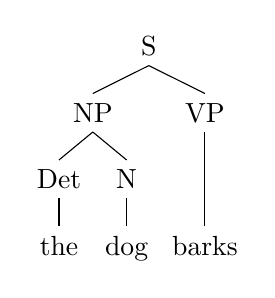
\begin{tikzpicture}
\tikzset{level 1+/.style={level distance=2\baselineskip}}
\tikzset{frontier/.style={distance from root=6\baselineskip}}
\Tree[.S
       [.NP 
         [.Det the ]
         [.N   dog ] ]
       [.VP barks ] ]
\end{tikzpicture}
}
\caption{\label{fig-example-fig-the-dog-barks}An example of a figure: Analysis of the sentence \emph{The dog barks.}}
\end{figure}

\begin{table}[htbp]
\caption{\label{tab-example-croft}An example of a table taken from \citew[214]{Croft2003a}}
\centerline{
\begin{tabularx}{\textwidth}{llX}\hline\hline
          & Low categoriality unit      & Unit with wich it clusters\\\hline
`Noun'    & low referentiality NP       & forgrounded verb\\
          & attached body part noun     & forgrounded verb\\
          & anaphoric NP                & forgrounded verb, emphasized element\\
`Verb'    & tense/aspect/mood auxiliary & forgrounded verb\\ 
\hline\hline
\end{tabularx}
}
\end{table}

\section{Footnotes}

Notes are footnotes rather than endnotes. Footnote numbers go to the end of the clause after punctuation
unless they refer to a specific word or phrase.\footnote{
  This is an example of a footnote that refers to the whole clause.
}

Footnote numbers should not be used in tables or figures\footnote{
  This is a footnote that refers to the word \emph{figures}. 
} but should be attached to the text preceding or following them.

\inlinetodostefan{Martin: [COMMENT: Manchmal braucht man solche Tabellen-internen Fußnoten; dann verwendet man manchmal Buchstaben a, b, c als Fußnotenzeichen]}


\section{Quotations}

If long passages are quoted, they should be indented and the quote should be followed by the exact reference. Use the quotation environment \latex provides:
\begin{quotation}
Precisely constructed models for linguistic structure can play an
important role, both negative and positive, in the process of discovery 
itself. By pushing a precise but inadequate formulation to
an unacceptable conclusion, we can often expose the exact source
of this inadequacy and, consequently, gain a deeper understanding
of the linguistic data.
\citep[5]{Chomsky57a}
\end{quotation}
%
Short passages should be quoted inline using quotes: \citet[5]{Chomsky57a} stated that ``[o]bscure
  and intuition-bound notions can neither lead to absurd conclusions nor provide new and
correct ones''.

If you quote text that is not in the language of the book provide a translation. Short quotes should
be translated inline, long quotes should be translated in a footnote.

\section{Cross-references in the text}

Please use the cross-referencing mechanisms of your text editing/type setting software. Using such
cross-referencing mechanisms is less error-prone when you shift text blocks around and in addition
all these cross-references will be turned into hyperlinks between document parts, which makes the
final documents much more useful.

If you have numbered example sentence, please start with (1) for every new chapter.
%%
%% Alternatively, you may put the chapter number in front of the example number (thus starting with (7.1), (7.2), ... in chapter 7, for example).
%% [COMMENT: Bei Grammatiken ist es durchaus üblich, dass alle Beispiele im Buch durchnummeriert werden. Auch in Rießlers Arbeit sind die Beispiele komplett durchnummeriert. Ich bin mir nicht sicher, wie wichtig diese Regelung ist, und ob wir nicht Volldurchnummerierung auch erlauben sollten.]

Please use capitals if you refer to numbered chapters, sections, tables, figure, or footnotes: \emph{As we have shown in
  Section~3.1}, \emph{As Figure~3.5 shows}. Do not capitalize without a number: \emph{In the
  following section we will discuss}.
Depending on the series and the langauge the book is published in authors may also use the § sign
instead of the word \emph{Section}. So the above sentence would read: \emph{As we have shown in
  §3.1}.

\section{Citations and references}
\label{sec-references-authors}

A citation is author-year information (optionally with page number or other more detailed information) in the text. A bibliographical reference is metadata about a work that is cited.

If books or larger articles are cited for a smaller point, exact page numbers should be provided. This is a good service to the readers, and it is also good for
authors since it helps them to keep track of their source and enables them to find and reread the
referenced passages and it is a good service to the readers.

For references in the bibliography, we use the \emph{Unified Style Sheet for Linguistics},\footnote{\url{http://celxj.org/downloads/UnifiedStyleSheet.pdf}}. The \bibtex file is contained in the \latex
classes that are used for typesetting \lsp books. 
Please deliver a \bibtex file with all your references together with your submissions. 
\bibtex can be exported from all common bibliography tools (We recommend BibDesk for the Mac and JabRef for all other platforms). 
Please make sure that all \bibtex fields are complete. %what is the reference of  `all'? each and every imaginable bibtexfield?
Please provide all first and last names of all authors and editors. Do not use et~al. in the Bibtex file; this will be generated automatically when inserted.
For bipartite family names like ``von Stechow'', ``Van Eynde'', and ``de Hoop'' make sure that these
family names are contained in curly brackets. These authors will then be cited as
\citet{VanEynde2006a} and \citet{vonStechow84a}. Note that Dutch names like ``de Hoop'' are not treated differently from other surnames.

The references in your \bibtex file will automatically be correctly typeset. So, provided the
\bibtex file is correct, authors do not have to worry about this. But there are some things to
observe in the main text. Please cite as shown in Table~\ref{tab-citation}.

\begin{table}[htbp]
\caption{\label{tab-citation}Citation style for \lsp}
\centerline{%
\begin{tabular}{lp{9cm}}\hline\hline
citation type & example\\\hline
author & As \citet[215]{MZ85a} have shown\\
       & As \citet[215]{MZ85a} and \citet{Bloomfield33a} have shown\\
work   & As was shown in \citew[215]{Saussure16a}, this is a problem for theories that \ldots\\
work   & This is not true \citep{Saussure16a,Bloomfield33a}.\\\hline\hline
\end{tabular}
}
\end{table}
\nocite{Bresnan82b}% something with an editor.

Citations consist of author name plus year number in parentheses (with page number or other information). There is no comma between the author name and the year number. If a citation is itself in parentheses, the parentheses around the year number are omitted (unless there is a fairly long text in the parentheses, in addition to the citation).

%% Table~\ref{tab-various-publication-types} provides examples for different publication types (book,
%% journal article, paper in an edited volume, and so on). Please refer to the bibliography at the end
%% of this book to see how the respective items are formated.

If you have an enumeration of references in the text as in \emph{As X, Y, and Z have shown}, please use
the normal punctuation of the respective language rather than special markup like `;'.

If you refer to regions in a text, for instance 111--112, please do not use 111f.\ or 111ff.\ but provide the
full information. 

\noindent
\inlinetodostefan{Say something about decapitalization. \url{http://tex.stackexchange.com/a/140071/12092}}

\section{Special terms}

If you refer to special terms, please use italics as in ``I 
use the term \emph{nominative} for \ldots



\section{Punctuation}
Please use punctuation consistently. 
If you use initial adverbial clauses, please use commas: When referring to such nominatives, I use {\ldots}.
EN-dashes are used for ranges (e.g. 1985–1995).

\section{Academic \emph{we}}

Monographs and articles that are authored by a single author should use the pronoun \emph{I} rather
than \emph{we} as in ``As I have shown in Section~3''.	

\section{Special guidelines for edited volumes}


Some special rules apply to the chapter of edited volumes:
\begin{itemize}
\item Each paper has its own list of references (unnumbered section labeled References).
% \item Each paper should start with a short abstract
\item A paper may have a special unnumbered section Acknowledgements just after the last numbered section. This is preferable to putting the acknowledgements into the footnotes.
\item A paper may have a special unnumbered section Abbreviations (or similar) just before the References. This is strongly preferred to listing the abbreviations in a footnote.
\item Chapter numbers should not be used in numbering tables and figures within such chapters.
\end{itemize}


\section{Checklist}

The following is a general checklist for authors. Author who use \latex should also consult the
checklist for advanced authors/typesetters in Section~\ref{sec-check-typesetters}.

\section{Other}

Running heads:
\begin{itemize}
\item Monographs
left-hand side: chapter number and chapter heading 
right-hand side: section number and section heading
\item Edited volumes:
left-hand side: author name
right-hand side: (chapter number and) chapter name
\end{itemize}


%% -*- coding:utf-8 -*-
\chapter{\LaTeX}


\section{Installation of the \texttt{langsci} class}

The \latex class for typesetting Language Science Press books was developed by Timm
Lichte\ia{Lichte, Timm} with
help be Berthold Crysmann\ia{Crysmann, Berthold} and me\aimention{M\"uller, Stefan}. It can be downloded from the GitHUB\is{GitHUB} repository at: \url{https://github.com/langsci/latex}
You can download the classes directly from the given web page or use the following git commands to
create a local copy of the repository:
\begin{verbatim}
git init
git clone https://github.com/langsci/latex.git 
\end{verbatim}
If you are using \texttt{git}, you can update your installation by executing the following command:
\begin{verbatim}
git pull origin
\end{verbatim}

Place all files and subdirectories from this repository into your local working directory.

\section{Using the \texttt{langsci} class}

Once you installed the classes in your system, you may look at the file \texttt{test.tex} to see how
a book can be typeset. The code of this book is available in the directory \texttt{Guidelines}. Once
you set up your \latex files you can compile them by calling 
\begin{verbatim}
xelatex yourfilename.tex
\end{verbatim}

%\DescribeMacro{\BackTitle}


\subsection{Class options}

A \latex document starts with a specification of a document class. Usually this is a class for
books, articles, or technical reports. \lsp has a special class that is called \texttt{langsci} and is
based on the book class from the KomaScript package. Several options can be passed to the class. The
following code shows how the class is loaded and how options are set. 


\begin{verbatim}
\documentclass[series=labphon,
               number=1,
               isbn=978-3-944675-01-5,
               url=http://langsci-press.org/catalog/book/16,
               output=long]{langsci}            
\end{verbatim}

The options are explained in the following paragraphs.


\subsubsection{\texttt{series}}

The\isoption{series} name of the series in which a book is published has to be passed to the langsci package. This will ensure that the name of
the series is put on the cover and the right color for your series will be
selected. Table~\vref{table-series} provides an overview of the series that are established as of
\today.
\begin{table}[htbp]
\caption{\label{table-series}Series of \lsp as of \today}
\centerline{%
\begin{tabular}{ll}\hline\hline
Option  & Full Name\\\hline
eotms   & Empirically Oriented Theoretical Morphology and Syntax\\
eotmsig & Implemented Grammars\\
sidl    & Studies in Diversity Linguistics\\
algad   & African Language Grammars and Dictionaries\\
tmnlp   & Translation and Multilingual Natural Language Processing\\
lnls    & Lecture Notes in Language Sciences\\
nc      & Monographs on Comparative Niger-Congo\\
labphon & Studies in Laboratory Phonology\\
\hline\hline
\end{tabular}
}
\end{table}



\subsubsection{\texttt{number}}

Authors\isoption{number} will be informed by their editor about the number that their book has in the series. This
number is passed with the \texttt{number} option to the langsci class.

\subsubsection{\texttt{isbn}}

Once\isoption{isbn} a manuscript is accepted, authors have to sign a publication agreement with the FU Library (see
Chapter~\ref{chap-publication}). Then they will get an ISBN, which has to be passed to the langsci class.

\subsubsection{\texttt{url}}

When\isoption{url} a manuscript is submitted to \lsp the submission gets a number and there will be a
corresponding URL. This URL has to be passed to the langsci class, since it will be part of the
copyright information of the book.

\subsubsection{\texttt{output}}

There\isoption{output} are three options for output: \texttt{long}, \texttt{short}, and \texttt{inprep}. If you pass
\texttt{long} to the langsci class, all pages are printed. This includes front and backpane of the
cover and also its spine. If the option \texttt{short} is used, the cover pages are omitted. This
document version is much more printer friendly since the colored pages are not included.

The option \texttt{inprep} suppresses everything that refers to \lsp. This gives authors the
possibility to write their book using the \lsp classes and styles prior to submission. They may then
distribute the manuscript without revealing their intention to submit to \lsp.

\subsubsection{\texttt{smallfont}}

\lsp\isoption{smallfont} books are typeset with an 11pt font. Those books that would be longer than 500 pages should be
typeset with the \texttt{smallfont} option, which selects a 10pt font.

\subsubsection{\texttt{draftmode}}

Since\isoption{draftmode} \lsp does not have any commercial interest you can put your book on webpages and distribute it
freely. We encourage authors to do this in order to discuss the work and improve it before final
publication. If authors want to circulate prefinal versions, they can use the option
\texttt{draftmode}. This prints a large watermark onto the first page and adds a footer to ever page
that informs the reader about the fact that he is reading a draft and the date and time of the
creation of the draft.


\subsubsection{\texttt{copyright}}

Usually \lsp books are published under the Creative Commons license CC-BY. However, there are rare
cases where other licenses are required (for instance for translations of books that were published
with another publisher who has the rights for the original version). For such cases, there is the
\isoption{copyright} the \texttt{copyright} option. One can pass any other CC license string to the
\latex class in the following way:
\begin{verbatim}
copyright=CC-BY-ND
\end{verbatim}


\subsection{Commands}

You can specify a title with the \verb+\title+\iscommand{title} command (\latex standard). In addition the langsci
class provides a command for specifying a subtitle (\verb+\subtitle+\iscommand{subtitle}). The author of a book is
specified by \verb+\author+\iscommand{author}. A separate page with a dedication can be inserted by \verb+\dedication+\isoption{dedication}.

The title of the book that goes to the back of the book is specified by \iscommand{BackTitle}\verb+\BackTitle+ and the
cover text on the back is provided by \verb+\BackBody+\iscommand{BackBody}.


\section{Workflow}

\subsection{Compiling the document}
\label{sec-latex-compilation}

There are various tools for all existing platforms that help authors/typesetters compiling the
documents and creating indices and references. The following commands can be called explicitly from
the commandline in Unix-based systems:
\begin{fitverb}
xelatex -no-pdf yourfilename
bibtex -min-crossrefs=200 yourfilename
xelatex -no-pdf yourfilename
bibtex -min-crossrefs=200 yourfilename
xelatex yourfilename -no-pdf
correct-toappear
correct-index
makeindex -o yourfilename.ind yourfilename.idx
makeindex -o yourfilename.lnd yourfilename.ldx
makeindex -o yourfilename.wnd yourfilename.wdx
LSP/bin/reverse-index <yourfilename.wdx >yourfilename.rdx
makeindex -o yourfilename.rnd yourfilename.rdx
\rm yourfilename.adx
authorindex -i -p yourfilename.aux > yourfilename.adx
sed -e 's/}{/|hyperpage}{/g' yourfilename.adx > yourfilename.adx.hyp
makeindex -o yourfilename.and yourfilename.adx.hyp
xelatex yourfilename
\end{fitverb}

\noindent
These commands do the following: they run the documents through \xelatex, call \bibtex, create the
indices using \texttt{makeindex}, and create a reverse index of expressions and an author index.

Everytime \xelatex is run it writes information about the sections and figures and son on auxiliary
files. These auxiliary files are read in when \xelatex runs again. They are used by \xelatex to create a
table of contents and by \bibtex to create the list of references. Due to the insertion of a table of
contents the page numbering may change. Therefore it is necessary to run \xelatex several times to
get a stable document.

We decided not to use the crossreferencing\is{crossreferencing} facility that \bibtex provides. Crossreferencing saves
space if several papers in the same edited volume are cited, but is opaque for indexing tools like
google scholar. Crossreferencing is disabled by the command option \verb+-min-crossrefs=200+ that is
passed to the \texttt{bibtex} command.

\subsection{Makefiles}

Of course nobody wants to type in the commands mentioned in Section~\ref{sec-latex-compilation} by
hand. Instead a Makefile\is{Makefile}\is{make} can be used. You will find an example Makefile in the
github repository in the directory that also contains the code for this book.\footnote{
  \url{https://github.com/langsci/latex/tree/master/Guidelines}, 16.02.2014.
}


\subsection{Using includes}

\subsection{Version control}


\section{Document structure}




\subsection{References}

\lsp uses the \texttt{natbib}\ispackage{natbib} package together with \bibtex\is{bibtex@\bibtex} and the \bibtex style \texttt{unified.bst}.


\subsection{Citation}

As was explained in Section~\ref{sec-references-authors} citations that provide a page number are
given required to be in the format Author (1975: 312) rather than Author (1975: p.\,312). If authors
want their text to be copy\&paste-proof, they can define the command \verb+\page+ and cite as
follows:
\begin{verbatim}
\citet[\page 312]{Author1975a}
\end{verbatim}
For \lsp \verb+\page+ would be:
\begin{verbatim}
\newcommand{\page}{}
\end{verbatim}
For other publications authors can use the following
\begin{verbatim}
\newcommand{\page}{p.\,}
\end{verbatim}
In case several pages are cited, the page numbers should be passed to cite as follows:
\begin{verbatim}
\citet[\page 312, 740, 756--758]{Author1975a}
\end{verbatim}


\subsection{Crossreferencing}

%% You may use \verb+(\mex{1})+\iscommand{mex} to refer to the following example and \verb+(\mex{0})+ to the preceeding
%% example. You can also pass smaller numbers or larger numbers to \verb+\mex+ but I would suggest not
%% to do this since often text blocks are inserted between the example and its description and then
%% references are broken. Furthermore t
The standard referencing mechanism creates hyperlinks to the
example sentences and depending on your viewer this gives you a nice preview of the referenced
material.
%, which you do not get with \verb+\mex+. 
See Figure~\vref{fig-preview-of-hyperlink-with-skim} for an example for such a preview.
\begin{figure}[htbp]
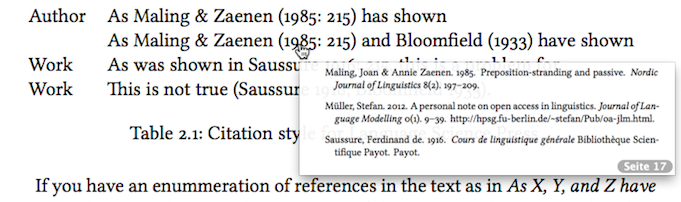
\includegraphics[width=\linewidth]{crossref.png}
\caption{\label{fig-preview-of-hyperlink-with-skim}Hyperlinked reference allow a preview in some viewers}
\end{figure}


There should not be a linebreak in something like \emph{Section~4}. This is achieved by using an explicit
whitespace: \verb+Section~\ref{sec-examples}+ This also makes sure that \latex is not inserting too
much space when material is distributed in a line.

\subsection{Indexes}

The\is{index|(} \lsp class is set up in a way that an author index is created automatically. If you want to add
an author that is not cited (for instance in the acknowledgements), you can do this by calling
\verb+\aimention{Zappa, Frank}+.\aimention{Zappa, Frank}\iscommand{aimention}

You may enter items into the subejct index by calling \verb+\is+, for example 
\begin{verbatim}
\is{word}
\end{verbatim}

Regions can be specified by appending \verb+|(+ to the keyword at the beginning of a region and
\verb+|)+ at the end of the region. For instance this section has the index entry
\verb+\is{index|(}+ after the first word of this section and \verb+\is{index|)}+ at the very end of
this section. If this rather brief section happens to be set on one page, \latex enters one page
number into the index. If there is a pagebreak in the middle of this section, a region is entered
into the index.

If you mention a language, you may add it to the language index: 
\begin{verbatim}
\il{Mandarin Chinese}
\end{verbatim}
If you are working in a theory that uses features (like LFG or HPSG), you may use \verb+\isfeat+ to enter
features into the subject index. \verb+\isfeat{comps}+\isfeat{comps} would enter the \compsf into the subject
index. The typesetting of the feature name in {\sc small caps} will be done automatically.

Words (or stems) can be entered into a special index by using \verb+\iw+. For instance,
\verb+\iw{Mann}+ enters the word \emph{Mann}\iw{Mann} in to the index of expressions.

Authors working in the area of morphology may find a reverse index of expressions useful. For
instance, if one wants to find all references to words ending on \suffix{ung} (as for instance \emph{Besprechung}\iw{Besprechung}, \emph{Lesung}\iw{Lesung},
\emph{Sitzung}\iw{Sitzung}, or \emph{Vorlesung}\iw{Vorlesung}), one can look them up
in the reverse index of expressions easily.

All these index commands can also be used in footnotes.\footnote{
  The commands are set up in a way that automatically distinguishes between index entries in
  footnotes and outside of footnotes. For instance the call of \texttt{$\backslash$iw\{Mann\}} for the word
  \emph{Mann}\iw{Mann} causes a special marking in the expression index.
}

All index entries are hyper-linked to the respective pages.

Indexes are inserted at the end of the document by specifying a subset of the following calls:
\begin{verbatim}
\clearpage
\pdfbookmark[0]{Index}{Index}
\pdfbookmark[1]{Expression index}{Expression index}
\printindex[wrd]
\pdfbookmark[1]{Reverse expression index}{Reverse expression index}
\printindex[rwrd]
\pdfbookmark[1]{Name index}{Name index}
\printindex[aut]
\pdfbookmark[1]{Language index}{Language index}
\printindex[lan]
\pdfbookmark[1]{Subject index}{Subject index}
\printindex
\end{verbatim}

While working at a manuscript it can be practical to see index entries in the margins. Index entries may be
switched on by specifying \verb+\proofmodetrue+ in the preamble of the
document.\iscommand{proofmodetrue} The following specification checks whether the option
\texttt{draftmode}\isoption{draftmode} of the \texttt{langsci} is used and displays the index entries in the margin if
this is the case:
\begin{verbatim}
\iflsDraft
\proofmodetrue
\fi
\end{verbatim}


\is{index|)}

\subsection{Hyphenation}

There is a special draft mode that can be used for the preparation of manuscripts. It can be enabled
by passing the option \texttt{draftmode} to the langsci class. In draftmode words that could not be
hyphenated automatically stick out in the right margin. Such problematic words are marked with a
black box so that they can be detected easily. You can fix such problems by inserting explicit
hyphenation rules in a word. This is done by \verb+\-+, for example \verb+weath\-er+. However, this
method is dispreferred since it only affects one occurrence of the word rather than all occurrences in
the current and further documents. The right way to deal with hyphenation issues is to put your
hyphenation preferences into a file and include this file in all your publications. 

\begin{verbatim}
\hyphenation{
Ajd-ukie-wicz
Prze-piór-kow-ski
To-ma-sel-lo
To-ron-to
trans-for-ma-tions-gram-ma-ti-sches
Tü-bing-en
Um-welt-ver-gif-tung
Ver-lags-buch-hand-lung
West-deut-scher
Wis-sen-schaft-liche
weath-er
}
\end{verbatim}

%xxx xxxxxxxxxxxxxxxxx xxxxxxxxxxxx xxx xxxxxxxxxx xxxxxxxxxxx Wirtschaftswunder.
%
%xxx xxxxxxxxxxxxxxxxx xxxxxxxxxxxx xxx xxxxxxxxxx xxxxxxxxxxx Wissenschaftliche.



\section{Packages specific for linguistics}

There is a huge amount of packages that can be used for various purposes. \citew{MG2013a} is a good
reference book. This section discusses some aspects of some packages that are relevant for
linguistics. Every \latex package comes with a documentation and users should consult these
documentations too. The purpose of this section is to point users to the packages that we think
serve their purpose best and that are compatible with other packages and the \lsp classes, as this
book proves.

\subsection{Glossed examples}

Glossed\is{glossing|(}\ispackageb{lsp-gb4e} examples are typeset with a modified version of the \texttt{gb4e}\ispackage{gb4e} package by Craig
Thiersch\aimention{Thiersch, Craig}. The modified package is called \texttt{lsp-gb4e}. It is contained in the styles directory
that is delivered with the \lsp \latex calsses. It differs from the original package in loading a
version of \texttt{gloss} that was modified by Alexis Dimitriadis\aimention{Dimitriadis, Alexis} in order to be compatible with
\texttt{jambox} (see Section~\ref{sec-jambox}).

Simple examples like (\mex{1}) can be typeset as shown below.
\ea
\iw{Mann}\iw{schlafen}
\gll Der Mann schläft.\\
     the man  sleeps\\
\glt `The man sleeps.'
\z
\begin{verbatim}
\ea
\gll Der Mann schläft.\\
     the man  sleeps\\
\glt `The man sleeps.'
\z
\end{verbatim}
Lists of examples can be typeset with \verb+\eal+ and \verb+\zl+ respectively. The example in
(\mex{1}) shows how the sentences can be aligned properly:
\eal
\ex[]{
\iw{Linguist}\iw{Nobelpreis}\iw{glauben}
\gll Ich glaube dem Linguisten nicht, einen Nobelpreis gewonnen zu haben.\\
     I believe the linguist not a Nobel.prize won to have\\
\glt  `I don't believe linguist's claim that he won a Nobel prize.'
}
\ex[*]{
\gll Dem Linguisten einen Nobelpreis  glaube  ich nicht gewonnen zu haben.\\
     the linguist   a     Nobel.price believe I   not   won      to have\\
}
\zl
\begin{fitverb}
\eal
\ex[]{
\gll Ich glaube  dem Linguisten nicht, einen Nobelpreis  gewonnen zu haben.\\
     I   believe the linguist   not    a     Nobel.prize won      to have\\
\glt  `I don't believe linguist's claim that he won a Nobel prize.'
}
\ex[*]{
\gll Dem Linguisten einen Nobelpreis  glaube  ich nicht gewonnen zu haben.\\
     the linguist   a     Nobel.price believe I   not   won      to have\\
}
\zl
\end{fitverb}

If you want to add a footnote\is{footnote|(} that provides the source of an example as in (\mex{1}), you can do
this as follows:
\ea
\gll Piloten         fik frataget    sit certifikat\footnotemark\\
     pilot.{\sc def} got deprived.of his license\\
\footnotetext{KorpusDK.}
\glt `The pilot was deprived of his license to fly.'
\z 
\begin{verbatim}
\ea
\gll Piloten         fik frataget    sit certifikat\footnotemark\\
     pilot.{\sc def} got deprived.of his license\\
\footnotetext{KorpusDK.}
\glt `The pilot was deprived of his license to fly.'
\z 
\end{verbatim}
Please call the \verb+\footnotetext+ command before the translation, since otherwise the
footnotetext may be typeset on a page that is different from the one where the footnotemark is set.\is{footnote|)}

For the typesetting of an additional line with the original script, one may use \verb+\glll+ rather
than \verb+\gll+. (\mex{1}) shows a Chinese example:
\ea
\label{ex-chinese}
\glll 狗       叫     了。\\
      gou3     jiao4   le\\
      dog      bark    ASP/CRS\\
\glt `The dog is barking.'/`The dogs are barking.'
\z

\begin{verbatim}
\ea
\glll 狗       叫     了。\\
      gou3     jiao4   le\\
      dog      bark    ASP/CRS\\
\glt `The dog is barking.'/`The dogs are barking.'
\z
\end{verbatim}


In some subdisciplines of linguistics (e.\,g.\ typology) the examples are written in italics as in the
following example:
\ea
\def\exfont{\normalsize\it}
\gll Piloten         fik frataget    sit certifikat\footnotemark\\
     pilot.{\sc def} got deprived.of his license\\
\footnotetext{KorpusDK.}
\glt `The pilot was deprived of his license to fly.'
\z 
Authors do not have to care for this. The code for typesetting this is exactly the same as for the
variant without italics.
% of course this is not true for the code above ...
The series editor decided whether italics is used or not.

If the series decides to use italics, it has to be ensured that structural markup like brackets are
not typeset in italics:
\ea
\def\exfont{\normalsize\it}
\gll ein {\rm[}interessantes       Beispiel{\rm]}\\
     an  \hspaceThis{[}interesting example\\
\glt `an interesting example'
\z 
\begin{verbatim}
\ea
\gll ein {\rm[}interessantes       Beispiel{\rm]}\\
     an  \hspaceThis{[}interesting example\\
\glt `an interesting example'
\z 
\end{verbatim}
\is{glossing|)}\ispackagee{lsp-gb4e}
%% \inlinetodostefan{
%% The translation should not be separated from the glossed example by a page break.
%% }

In typological series examples often come with the language name and references. The examples on
page~\pageref{ex-typology} are typeset as follows:
\begin{verbatim}
\ea
{\rm Mising\il{Mising} \citep[69]{Prasad91a}}\\
\gll azɔ́në dɔ́luŋ\\
     small village\\ 
\glt `a small village' 
\z

\eal
\ex {\rm Apatani\il{Apanti} \citep[23]{Abraham85a}}\\
\gll aki atu\\ 
     dog small\\ 
\glt ‘the small dog’ 
\ex {\rm Temiar\il{Temiar} \citep[155]{Benjamin76a}}\\ 
\gll dēk mənūʔ\\
     house big\\
\glt ‘big house’ 
\zl
\end{verbatim}


\subsection{\texttt{jam\-box}}
\label{sec-jambox}


The\ispackageb{jam\-box} package \texttt{jambox} by Alexis Dimitriadis\aimention{Dimitriadis, Alexis} can be used to provide information about the language of an example or
about a certain other aspect to be highlighted.\il{Maltese}
\settowidth\jamwidth{VSO}
\eal
\ex[]{
\label{ex-ingrid-kielet-ilmazzita}
\gll Ingrid kiel-et il-mazzit-a.\\
     Ingrid eat-{\sc 3sg.f} {\sc def}-black.pudding-{\sc sg.f}\\ \jambox{(SVO)}
\glt `Ingrid ate black pudding.'
}
\ex[]{
Kielet ilmazzita Ingrid. \jambox{(VOS)}
}
\ex[*]{
Kielet Ingrid ilmazzita. \jambox{(VSO)}
}
\ex[]{\label{ex-sov}
Ingrid ilmazzita kielet. \jambox{(SOV)}
}
\ex[]{\label{ex-osv}
Ilmazzita Ingrid kielet. \jambox{(OSV)}
}
\ex[]{
Ilmazzita kielet Ingrid. \jambox{(OVS)}
}
\zl

The call of \verb+\jambox+ has to follow the linebreak after the gloss:
\begin{verbatim}
\ex[]{
\label{ex-ingrid-kielet-ilmazzita}
\gll Ingrid kiel-et il-mazzit-a.\\
     Ingrid eat-3fsg def-black.pudding-fsg\\ \jambox{(SVO)}
\glt `Ingread ate black pudding.'
}
\end{verbatim}
The distance from the right margin can be specified by passing the largest object to be placed in a
jambox to \verb+\settowidth+:

\eal
\settowidth\jamwidth{(German)}
\ex The man reads the book.    \jambox{(English)}
\ex Manden læser bogen.        \jambox{(Danish)}
\ex Der Mann liest das Buch.   \jambox{(German)}
\zl

\begin{verbatim}
\eal
\settowidth\jamwidth{(German)}
\ex The man reads the book.    \jambox{(English)}
\ex Manden læser bogen.        \jambox{(Danish)}
\ex Der Mann liest das Buch.   \jambox{(German)}
\zl
\end{verbatim}
\ispackagee{jam\-box}



\subsection{Trees: \texttt{tikz-qtree}}

Several\ispackageb{tikz-qtree} tree-drawing packages are around and all have their advantages and disadvantages. I
used \texttt{tree-dvips} for decades, but it is incompatible with \xelatex, since it creates
PostScript rather than PDF. Exploring the options I discovered \texttt{tikz-qtree}, which is a
tikz-based\ispackage{tikz} reimplementation of Alexis Dimitriadis'\aimention{Dimitriadis, Alexis} \texttt{q-tree}
package. The syntax for drawing trees is rather simple and in comparison to \texttt{tree-dvips} drawing trees
is considerably speeded up. Figure~\vref{fig-the-dog-barks} shows a simple example.
\begin{figure}[htbp]
\centerline{%
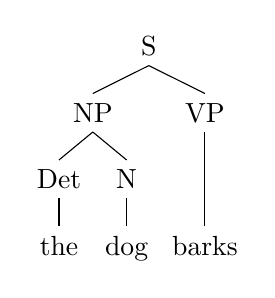
\begin{tikzpicture}
\tikzset{level 1+/.style={level distance=2\baselineskip}}
\tikzset{frontier/.style={distance from root=6\baselineskip}}
\Tree[.S
       [.NP 
         [.Det the ]
         [.N   dog ] ]
       [.VP barks ] ]
\end{tikzpicture}
}
\caption{\label{fig-the-dog-barks}Tree for \emph{The dog barks.} drawn with \texttt{tikz-qtree}}
\end{figure}
\begin{fitverb}
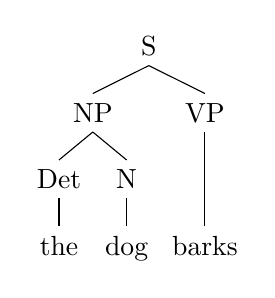
\begin{tikzpicture}
\tikzset{level 1+/.style={level distance=2\baselineskip}}
\tikzset{frontier/.style={distance from root=6\baselineskip}}
\Tree[.S
       [.NP 
         [.Det the ]
         [.N   dog ] ]
       [.VP barks ] ]
\end{tikzpicture}
\end{fitverb}

The code below shows how words below a certain node can be put under a triangle as in Figure~\vref{fig-the-dog-barks-abbreviated}.
\begin{figure}[htbp]
\centerline{%
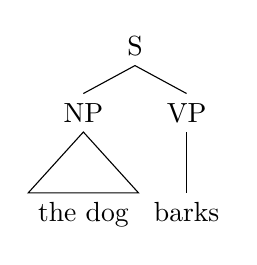
\begin{tikzpicture}
\tikzset{level 1+/.style={level distance=2\baselineskip}}
\tikzset{frontier/.style={distance from root=5\baselineskip}}
\Tree[.S
       [.NP  \edge[roof]; {the dog} ]
       [.VP barks ] ]
\end{tikzpicture}
}
\caption{\label{fig-the-dog-barks-abbreviated}Tree for \emph{The dog barks.} with abbreviated NP}
\end{figure}

\begin{samepage}
\begin{fitverb}
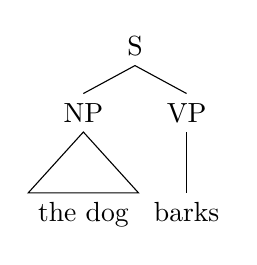
\begin{tikzpicture}
\tikzset{level 1+/.style={level distance=2\baselineskip}}
\tikzset{frontier/.style={distance from root=5\baselineskip}}
\Tree[.S
       [.NP  \edge[roof]; {the dog} ]
       [.VP barks ] ]
\end{tikzpicture}
\end{fitverb}
\end{samepage}
\ispackagee{tikz-qtree} 

\subsection{DRSes: \texttt{drs}}

DRSes\ispackageb{drs} can be typeset using the \texttt{drs} package by Alexis Dimitriadis\aimention{Dimitriadis, Alexis
}. There are various commands that let you typeset simple DRSes, ones with implications
and DRSes with quantifiers. Some examples from the manual are given below:

\bigskip

\drs{x y}{Jones(x) \\ Ulysses(y) \\ x owns y}

\begin{verbatim}
\drs{x y}{Jones(x) \\ Ulysses(y) \\ x owns y}
\end{verbatim}


\drs{x}{Jones(x) \\
      \ifdrs{y}{donkey(y)\\x owns y}
            {z w}{z = x\\ w = y\\ z feeds w}}

\begin{verbatim}
\drs{x}{Jones(x) \\
      \ifdrs{y}{donkey(y)\\x owns y}
            {z w}{z = x\\ w = y\\ z feeds w}}
\end{verbatim}

\drs{X}{ the lawyers(X) \\
        \qdrs{x}{x $\in$ X}
             {every}{x}
             {y}{secretary(y) \\ x hired y}}

\begin{verbatim}
\drs{X}{ the lawyers(X) \\
        \qdrs{x}{x $\in$ X}
             {every}{x}
             {y}{secretary(y) \\ x hired y}}
\end{verbatim}
\ispackagee{drs}

%%%%%%%%%%%%%%%%%%%%%%%%%%%%%%%%%%%%%%%%%%%%%%%%%%%%%%%%%%%%%%%%%%%%%%%%%%%%%%%%%%%%%%%%%%%%%%%%%%%

\subsection{AVMs}

The package for typesetting AVMs that is most widely used is the package \texttt{avm}\ispackage{avm}
by Chris Manning\aimention{Manning, Chris}. 

%% This package is described in the following
%% subsection. Section~\ref{sec-lsp-avm} describes AVM macros that were put together by Markus Duda\aimention{Markus Duda}.

%% \subsubsection{\texttt{avm}}

(\mex{1})\ispackageb{avm} shows an example of an AVM typeset with the \texttt{avm} package:
\ea
\label{ex-avm-avm}
\begin{avm}
\[phon   & \< {\it porcupine\/} \>\\
  feat-a & \@{10} \[feat-aa & type-aa\\
                    feat-ab & \< \[ synsem|loc|cat|head & type-aba\\
                                    feat-abc \tpv{type-abc} 
                                  \],
                                  \textup{NP} \>\\
                    \tp{type-a}
                  \]\\
 feat-b & \@{10} type-b\\ 
 \tp{some-type}
\]
\end{avm}
\z



\begin{verbatim}
\begin{avm}
\[phon   & \< {\it porcupine\/} \>\\
  feat-a & \@{10} \[feat-aa & type-aa\\
                    feat-ab & \< \[ synsem|loc|cat|head & type-aba\\
                                    feat-abc \tpv{type-abc} 
                                  \],
                                  \textup{NP} \>\\
                    \tp{type-a}
                  \]\\
 feat-b & \@{10} type-b\\ 
 \tp{some-type}
\]
\end{avm}
\end{verbatim}
%
The command \verb+\tp+ is defined as follows (the code is taken from Detmar
Meurers'\aimention{Meurers, Detmar} \texttt{avm+}\ispackage{avm+}):
\begin{verbatim}
% command to fontify the type values of an avm 
\newcommand{\tpv}[1]{{\avmjvalfont #1}}

% command to fontify the type of an avm and avmspan it
\newcommand{\tp}[1]{\avmspan{\tpv{#1}}}
\end{verbatim}

A more complex example is given in (\mex{1}):
\ea
\label{ex-avm-avm}
  \begin{avm}
    {\it word\/} $\rightarrow$
    \[ morphs & $\@{e_1}\bigcirc\cdots\bigcirc\@{e_n}$\\
       morsyn & \@0 $(\@{m_1}\uplus\cdots\uplus\@{m_n})$\\
       rules  & \< \[ morphs & \@{e_1}\\
                      mud & \@{m_1}\\ 
                      morsyn & \@0\], \ldots ,
                    \[morphs & \@{e_n}\\
                      mud    & \@{m_n}\\ 
                      morsyn & \@0\] \>
    \]
  \end{avm}
\z


The code is given below:
\begin{verbatim}
  \begin{avm}
    {\it word\/} $\rightarrow$
    \[ morphs & $\@{e_1}\bigcirc\cdots\bigcirc\@{e_n}$\\
       morsyn & \@0 $(\@{m_1}\uplus\cdots\uplus\@{m_n})$\\
       rules  & \< \[ morphs & \@{e_1}\\
                      mud & \@{m_1}\\ 
                      morsyn & \@0\], \ldots,
                    \[morphs & \@{e_n}\\
                      mud    & \@{m_n}\\ 
                      morsyn & \@0\] \>
    \]
  \end{avm}
\end{verbatim}
With the \texttt{avm} package it is possible to use brackets as they are used in AVMs.

The package has a good documentation and we will not repeat all the details here.
\ispackagee{avm}

%% \subsubsection{\texttt{lsp-avm}}
%% \label{sec-lsp-avm}

%% An alternative way to typeset AVMs is provided in the \lsp style file \texttt{lsp-avm} that contains
%% code by Markus Duda\aimention{Markus Duda} with some adaptions by Stefan Müller\aimention{Stefan
%%   M{\"u}ller}. The AVM in (\ref{ex-avm-avm}) is typeset as follows:

%% \ea
%% \ms[some-type]{
%%   phon   & \phonliste{ porcupine } \\
%%   feat-a & \ibox{10} \ms[type-a]{ feat-aa & type-aa\\
%%                                   feat-ab & \liste{ \onems{ synsem|loc|cat|head \type{type-aba}\\
%%                                                             feat-abc \type{type-abc} },
%%                                   NP }\\ }\\
%%  feat-b & \ibox{10} type-b\\ 
%% }
%% \z

%% %\ea
%% \begin{verbatim}
%% {\it word\/} $\rightarrow$
%%     \ms{ morphs & $\ibox{e_1}\bigcirc\cdots\bigcirc\ibox{e_n}$\\
%%          morsyn & \ibox{0} $(\ibox{m_1}\uplus\cdots\uplus\ibox{m_n})$\\
%%          rules  & \liste{ \ms{ morphs & \ibox{e_1}\\
%%                                mud & \ibox{m_1}\\ 
%%                                morsyn & \ibox{0} }, \ldots ,
%%                           \ms{ morphs & \ibox{e_n}\\
%%                                mud    & \ibox{m_n}\\ 
%%                                morsyn & \ibox{0} } }
%%       }
%% \end{verbatim}


\subsection{OT tableaux}


This\is{Optimality Theory|(}\is{tabular} section just provides some examples of how Optimality Tableaux can be typeset.

\begin{tabular}
       {|lc|c|c|c|}\hline   
      & \textbf{Input}  & Cnstrnt 1  &  Cnstrnt 2& Cnstrnt 3\\ \hline\hline
      & candidate 1     & *!         &           &          \\ \hline
      & candidate 2     &            &  *        &          \\ \hline
\hand & candidate 3     &            &           &  *       \\ \hline
\end{tabular}

\begin{fitverb}
\begin{tabular}
       {|lc|c|c|c|}\hline   
      & \textbf{Input}  & Cnstrnt 1  &  Cnstrnt 2& Cnstrnt 3\\ \hline\hline
      & candidate 1     & *!         &           &          \\ \hline
      & candidate 2     &            &  *        &          \\ \hline
\hand & candidate 3     &            &           &  *       \\ \hline
\end{tabular}
\end{fitverb}

\verb+\hand+ is defined as follows:

\begin{verbatim}
\usepackage{pifont}
\newcommand{\hand}{\ding{43}}
\end{verbatim}
 


\begin{tabular*}{0.95\textwidth}
    {@{\extracolsep{\fill}}|rl||c|c|c|}\hline   
      & \textbf{Input} & Constraint 1 & Constraint 2 & Constraint 3 \\ \hline\hline
      & candidate 1    & *!           &              &              \\ \hline
      & candidate 2    &              &  *           &              \\ \hline
\hand & candidate 3    &              &              &  *           \\ \hline
\end{tabular*}

\begin{fitverb}
\begin{tabular*}{0.95\textwidth}
    {@{\extracolsep{\fill}}|rl||c|c|c|}\hline   
      & \textbf{Input} & Constraint 1 & Constraint 2 & Constraint 3 \\ \hline\hline
      & candidate 1    & *!           &              &              \\ \hline
      & candidate 2    &              &  *           &              \\ \hline
\hand & candidate 3    &              &              &  *           \\ \hline
\end{tabular*}
\end{fitverb}

\begin{tabular}[t]{r|c|c|c|}
\cline{2-4}
      & /qi/  & qi    & qi         \\
\LCC 
      &       &       & \lightgray \\ \cline{2-4}
\hand & [qi]  &       & *          \\ \cline{2-4}
      & [*qi] & *!    &            \\ \cline{2-4}
\ECC
\end{tabular}


\begin{verbatim}
\usepackage{pstricks,colortab}

\begin{tabular}[t]{r|c|c|c|}
\cline{2-4}
      & /qi/  & qi    & qi         \\
\LCC 
      &       &       & \lightgray \\ \cline{2-4}
\hand & [qi]  &       & *          \\ \cline{2-4}
      & [*qi] & *!    &            \\ \cline{2-4}
\ECC
\end{tabular}
\end{verbatim}


\begin{tabular}{|l||c|c|} \hline
          &VO          &OV         \\ \hline\hline
\LCC
          &            &\lightgray \\ \hline
prefixing &Tagalog     &Ma'a       \\ \hline
\ECC
\LCC
           &\lightgray &            \\ \hline
suffixing  &Kwakwala   &Japanese    \\ \hline
\ECC
\end{tabular}

\begin{verbatim}
\begin{tabular}{|l||c|c|} \hline
          &VO          &OV         \\ \hline\hline
\LCC
          &            &\lightgray \\ \hline
prefixing &Tagalog     &Ma'a       \\ \hline
\ECC
\LCC
           &\lightgray &            \\ \hline
suffixing  &Kwakwala   &Japanese    \\ \hline
\ECC
\end{tabular}
\end{verbatim}
\is{Optimality Theory|)}



\subsection{Font issues and right to left scripts}

Since\is{font|(} we are using \xelatex, all fonts that are installed in the cannonical font directories can be
used. We are using the font \texttt{Linux Libertine}, which is unicode-based and contains a lot of
the characters linguists want to use.

\subsubsection{Chinese}
\label{sec-Chinese}

You can enter Chinese\il{Chinese}\is{Chinese Characters} characters directly and mix them with ASCII text without any further markup
provided you load the \texttt{xeCJK}\ispackage{xeCJK} package. We already saw an example in (\ref{ex-chinese}) on
page~\pageref{ex-chinese}. In order to type Chinese text, one has to load the \texttt{xeCJK} package
with the option \verb+indentfirst+ set to \verb+false+ and select an appropriate font:
\begin{verbatim}
\usepackage[indentfirst=false]{xeCJK}
\setCJKmainfont{SimSun}
\end{verbatim}


\subsubsection{Arabic script}

Arabic script\is{Arabic Script}\il{Persian} is the most challenging script for typesetting since it is written from right to left
and contains ligatures. If you load the \texttt{bidi} package, you can mix right to left and left to
right text.\footnote{
  Please have a look at the source code. The verbatim environment has difficulties to display Arabic
  text and hence the call to \texttt{$\backslash$PRL} comes out scrambled.
}

\ea
\PRL{او مرد را دوست نخواهد داشت.}\\
 \gll U      mard rā        dust   naxāhad        dāšt.\\
      He/she man  {\sc dom} friend {\sc neg}.want have\\
\glt `He/she will not love the man.'
\z

%\begin{rtlverbatim}
%\usepackage{fontspec}
\begin{verbatim}
\newfontfamily\Parsifont[Script=Arabic]{XB Niloofar}
\usepackage{bidi}
\newcommand{\PRL}[1]{\RL{\Parsifont #1}}

\ea
\PRL{او مرد را دوست نخواهد داشت.}\\
\gll U      mard rā       dust   naxāhad        dāšt.\\
     He/she man {\sc dom} friend {\sc neg}.want have\\
\glt `He/she will not love the man.'
\z
\end{verbatim}
%\end{rtlverbatim}

\subsubsection{Hebrew}

Hebrew\il{Hebrew|(} is also written from right to left. The characters are part of Linux Libertine, so no extra
font has to be loaded to set examples like (\mex{1}):
\ea
\RL{האישה קוראת ספר.}\\
\gll   ha-'iša          qore't                            sefer.\\
       {\sc def}-woman  read.{\sc pres}.{\sc f}.{\sc sg}  book\\
\glt `The woman is reading a book.'
\z
\begin{fitverb}
\ea
\RL{האישה קוראת ספר.}\\
\gll   ha-'iša          qore't                            sefer.\\
       {\sc def}-woman  read.{\sc pres}.{\sc f}.{\sc sg}  book\\
\glt `The woman is reading a book.'
\z
\end{fitverb}
\il{Hebrew|)}

\subsubsection{IPA symbols}

The\is{IPA symbols|(} IPA symbols are part of the Linux Libertine font and hence can be entered into the document
directly. The IPA unicode symbols can be created online at
\url{http://ipa.typeit.org/full/}. (\mex{1}) shows some examples:
\ea
ɓ ɐ ʁ ɾ ɻ ʃ ʂ θ~  t͡ʃ~  t͡s  ʈ ʊ ʊ̈ ʉ ʌ ʋ ʍ ɯ ɰ χ ʎ ɣ ʏ ɤ ʒ ʐ ʑ ʔ ʕ ʢ ʡ ɑ̃ ɔ ˧ ˨ ˩ ˩˥ ˥˩ ˦˥
\z
% ⱱ does not work  
If you find symbols that are not covered by the font, please use the \texttt{tipa} package.
\is{font|)}\is{IPA symbols|)}

\section{Bells and whistles}

\subsection{\texttt{varioref}}

\texttt{varioref}\ispackageb{varioref} is loaded by the \lsp class file. You can use \verb+\vref+\iscommand{vref} to refer to floating
objects like figures and tables. \latex automatically determines whether the floating object is on
the same page or further away. If the float is on the next page and the next page is to the right of
the current page, \latex will insert an appropriate text like \emph{on the facing page}. If we are
on a right page, \latex will insert something like \emph{on the next page} or \emph{on the facing page}. If the float is further
away, a page number will be provided.
\ispackagee{varioref}

%Please use \verb+\vref+ for the first reference to a float only.


\subsection{\texttt{german} for hyphenation}

If\is{hyphenation|(}\ispackageb{german} you write things like \verb+head-driven+ or very long paths like
{\sc snysem$|$""loc$|$""cat$|$""head$|$""mod$|$""loc}, \LaTeX{} does not do hyphenation
(in the part following the dash).

\verb+german.sty+ provides additional markup that allows for proper hyphenation:
\begin{verbatim}
head"=driven

{\sc snysem$|$""loc$|$""cat$|$""head$|$""mod$|$""loc}
\end{verbatim}
With this markup even long paths like {\sc snysem$|$loc$|$cat$|$""head$|$""mod$|$""loc$|$""cat$|$""head}
are typeset properly. Alternatively you my write
\begin{verbatim}
{\sc snysem$|$\-loc$|$\-cat$|$\-head$|$\-mod}
\end{verbatim}
which introduces a dash at the place of the linebreak:
{\sc snysem$|$\-loc$|$\-cat$|$\-head$|$\-mod$|$\-loc$|$\-cat$|$\-head}.

If you use \verb+german.sty+ for a book whose primary language is not German, do not forget to
specify the language you are using. For example, if your book is in US English you have to specify
the following:
\begin{verbatim}
\selectlanguage{USenglish}
\end{verbatim}
Otherwise the section name for references comes out in German.
\is{hyphenation|)}\ispackagee{german}

\subsection{Resizing large objects}

Trees and AVMs often are too big to fit onto one page. The \texttt{langsci} comes with commands for
shrinking large objects. You may pass your complex object as an argument to \texttt{\oneline} and
this will scale the object to \verb+\linewidth+ (the remaining space on the current line). There is
a more clever version of this command: \verb+\centerfit+. This command checks whether there is
enough space for an object and if this is the case it centers it in the line. If the object is
larger than the \verb+\linewidth+, it is resized to fit the line. This is very handy for typesetting
figures. You may copy and paste figures to other documents with a different text width without any
adaptations.


%% \begin{figure}[htb]
%% \centerfit{%
%% \begin{tikzpicture}
%% \tikzset{level 1+/.style={level distance=3\baselineskip}}
%% \tikzset{level 2+/.style={level distance=5\baselineskip}}
%% \tikzset{level 3+/.style={level distance=6\baselineskip}}
%% \tikzset{level 4/.style={level distance=7\baselineskip}}
%% \tikzset{level 5+/.style={level distance=5\baselineskip}}
%% \tikzset{frontier/.style={distance from root=26\baselineskip}}
%% %% \Tree[.{\ms[np-passive-cx]{ vform & passive \\
%% %%                             subj & \sliste{ NP\ind{1} }\\[2mm]
%% %%                             comps & \sliste{ (PP[\type{by}]\ind{2}) }\\
%% %%                           } }
%% %%         \ms{ vform & psp \\
%% %%              subj & \sliste{ NP\ind{2} }\\[2mm]
%% %%              comps & \sliste{ NP\ind{1} } 
%% %%            } ]
%% \Tree[.S
%%        [.{\ibox{1} NP\ind{2}} \edge[roof]; {the boy} ]
%%        [.VP\feattab{
%%                  \subj  \sliste{ \ibox{1} NP\ind{2} },\\
%%                  \comps  \sliste{  }}
%%          [.V\feattab{
%%                  \subj  \sliste{ \ibox{1} NP\ind{2} },\\
%%                  \comps  \sliste{ \ibox{3} }} was ]
%%          [.{\ibox{3} VP\feattab{
%%                  \vform \type{passive},\\
%%                  \subj  \sliste{ \ibox{1} NP\ind{2} },\\
%%                  \comps  \sliste{ }}} \edge node[auto=left]{Passive Construction};
%%            [.V\feattab{
%%                  \vform \type{psp},\\
%%                  \subj  \sliste{ NP },\\
%%                  \comps  \sliste{ NP\ind{2} }} 
%%              [.V\feattab{
%%                  \vform \type{psp},\\
%%                  \subj  \sliste{ NP },\\
%%                  \comps  \sliste{ NP\ind{2}, \ibox{4} }} given ] \edge node[auto=left]{Schema for Passive Participles};
%%              [.{\ibox{4} NP} \edge[roof]; { the ball } ] ] ] ] ] 
%% \end{tikzpicture}
%% }
%% \caption{\label{fig-the-boy-was-given-the-ball-tseng}Analysis of \emph{The boy was given the ball} according to \citet{Tseng2007a}}
%% \end{figure}


\subsection{Rotating figures and tables}
 

\subsection{\texttt{xspace} and abbreviations}

\ispackage{xspace}

\subsection{\texttt{todonotes}}

\ispackage{todonotes}

%% \section{Software}

%% \begin{itemize}
%% \item BibDesk
%% \item JabRef
%% \end{itemize}


\subsection{Style files and multiple projects}

Paths, shell variables \ldots

\section{Things you should not do}

\begin{itemize}
\item Please do not use explicit line breaks to mark a new paragraph. Paragraphs are marked by an empty
line in the text.
%\item Please do not 
\end{itemize}

\section{Checklist for typesetters/authors using \latex}
\label{sec-check-typesetters}

\begin{itemize}
\item Does your book compile without error messages? (Sounds trivial, but some tools just skip
  \latex errors)
\end{itemize}


%      <!-- Local IspellDict: en_US-w_accents -->

%% -*- coding:utf-8 -*-
\chapter{Publication}
\label{chap-publication}
\label{sec-license}

Language Science Press books are published on the Document Server of the Freie Universität Berlin
together with a print-on-demand option.


Authors have to make sure that they have permission to use copyrighted material from journals or
other books. A respective declaration is part of the submission process.






\backmatter

\bibliography{lsp-abbrev,lsp-guidelines}

%\cleardoublepage

\clearpage
\pdfbookmark[0]{Index}{Index}
\pdfbookmark[1]{Expression index}{Expression index}
\printindex[wrd]
\pdfbookmark[1]{Reverse expression index}{Reverse expression index}
\printindex[rwrd]
\pdfbookmark[1]{Name index}{Name index}
\printindex[aut]
\pdfbookmark[1]{Language index}{Language index}
\printindex[lan]
\pdfbookmark[1]{Subject index}{Subject index}
\printindex

                              
\end{document}
      
%      <!-- Local IspellDict: en_US-w_accents -->



On 19/03/2014 15:24, Sebastian Nordhoff wrote:
> da kann man noch ganz viele Sachen eintragen, zB Zielgruppe, Rechte etc
> (derzeit alles blank). Gibt es dafür schon einen Prozess? Sollen die
> Autoren hier Vorschläge machen, die Herausgeber, oder die Techniker (aka
> SN)?
Autoren machen Vorschläge, Reihenherausgeber segnen ab, würde ich sagen.
> Ich würde mal vorschlagen, ich mache das jetzt für Corinna nach bestem
> Wissen und Gewissen, aber in Zukunft sollten diese Dinge einheitlich
> geregelt sein
Genau, das muss ein Punkt in den Guidelines werden.

Aber wo genau erscheint diese Info?

M.



Würde ich nicht so streng sehen, aber ich persönlich habe eine Präferenz für "The term accusative" (also kursiv). Dann kann man die allgemeinen Regeln formulieren:

– Kursiv für metasprachliche Verwendung
– doppelte Anführungszeichen für Distanzierung (was andere sagen: Zitate, und von anderen verwendete Termini)
– einfache Anführungszeichen für Bedeutungen

(Stefan: Mir ist unklar, ob etwas davon in die allgemeinen LangSci-Guidelines rein soll. Bei manchen
dieser Dinge gibt es einfach unterschiedliche Konventionen.)


> Machst Du das weiter? Ich würde sonst alles einfach so an Corinna
> forwärtsen.
Hab gerade an Corinna geschrieben. Stefan, du kannst entscheiden, welche von diesen Dingen noch in
> die Guidelines rein sollen (eventuell, dass Termini kursiv sein sollen?, oder dass nach e.g. kein
> Komme kommt?). 

FAQ:

Ich vermute, dass Du \mainmatter nicht verwendet hast.

Im github gibt es ein Repository lsp-books, wo die Bücher zur Endredaktion reinkommen. Das ist öffentlich, allerdings nicht googlebar. Wenn Du willst, kann ich Dein Werk schon mal reinstellen. Dann haben alle Zugriff.


